\documentclass[fontset=windows,a4paper,12pt]{ctexart}
\usepackage{geometry}
\usepackage{graphicx}
\usepackage{subfigure}
\usepackage{graphics}
%\usepackage{overcite}
\usepackage{url}
\usepackage{listings}
\usepackage{CJK}

\pagestyle{plain}
\usepackage{bm}
\usepackage{amsmath}
\usepackage{multirow}

\geometry{top=25mm,bottom=20mm,left=25mm,right=25mm}
\newcommand{\upcite}[1]{\textsuperscript{\textsuperscript{\cite{#1}}}}
\renewcommand{\eqref}[1]{公式 (\ref{#1})}
\renewcommand*{\baselinestretch}{1.38}

\begin{document}
  \begin{center}
  	\zihao{3}{\heiti 小区开放对道路通行的影响}
  \end{center}
  \linespread{1.2}
  \begin{center}
  	\zihao{4}{\heiti 摘\ \ \ \ 要}
  \end{center}
  \zihao{4}{\songti 
  	
  	摘要摘要摘要摘要
  	摘要摘要摘要摘要
  	摘要摘要摘要摘要
  	摘要摘要摘要摘要
  	摘要摘要摘要摘要

  }
  \textbf{关键词:}\ 层次分析\ 元胞自动机
  
  \section{问题重述}
	基于“适用、经济、绿色、美观”的理念,为塑造城市良好风貌,缓解城市交通压力,促进土地节约利用,实现内部道路公共化,实现城市有序建设、适度开发、高效运行,近来,国务院发布的《关于进一步加强城市规划建设管理工作的若干意见》中指出,原则上不允许再建设封闭式小区,已建成的单位大院和住宅小区要逐步实现开放。此政策的颁布,引起了广泛的关注和讨论。

	然而小区由封闭型转向开放型,并非只拆除外部围墙就能达到。小区开放,即外部车辆可自由进出小区,小区内部道路作为市政道路使用。对此,大家产生疑惑:小区开放能否达到道路网结构优化,提高道路通行能力,改善交通状况的目的。如果小区开放能对周边道路通行能力起到改善效果,那么改善效果如何?对此,产生四种不同的观点:第一种观点认为,封闭型小区土地使用效率低,对土地分块化,破坏城市路网结构,堵塞路网结构中的“毛细血管”,增大路网压力,容易造成交通阻塞,不利于实现城市有序、高效建设的目标;第二种观点认为,小区开放增加了路网中道路数目,即路网密度增大,道路面积增加,通行能力自然有所提升;第三种观点认为,道路通行能力与小区位置、面积、内外部道路状况等诸多因素有关,不能一概而论小区开放产生的影响;还有一种观点认为,小区开放可以增加道路数量,但与此同时小区周边主路上进出小区交叉路口的车辆也相应的增加,可能会对主路的通行速度产生消极影响。

	现需要就小区开放对周边道路通行的影响进行研究,建立适当的数学模型并做定量分析,解决以下四个问题:
\begin{enumerate}
	\item 选取合适的评价指标体系,用以评价小区开放对周边道路通行的影响。
	\item 建立关于车辆通行的数学模型,用以研究小区开放对周边道路通行的影响。
	\item 小区开放产生的效果,可能会与小区结构及周边道路结构、车流量有关。选取或构建不同类型的小区,应用已建立的模型,定量比较各类型小区开放前后对道路通行的影响。
	\item 根据上述研究结果,从交通通行的角度,向城市规划和交通管理部门提出关于小区开放的合理化建议。
\end{enumerate}
  \section{符号说明}
  \section{问题分析}
  随着经济的发展,道路压力越来越大,我国现行的路网结构无法满足日益增长的车流量需求,而国外的小区开放制度对交通压力的缓解方式值得借鉴。根据对国内外开放小区与封闭小区数据的收集和对比,得到表\ref{tab:net_density}中的数据。
  \begin{table}[!htbp]
	\centering
	\caption{国际城市与国内城市路网密度对比\upcite{国外街区制是如何完美炼成}}
	\label{tab:net_density}
	\begin{tabular}{cc|cc}
		\hline 
		国内城市 & 路网密度($km/km^2$) & 国际城市 & 路网密度($km/km^2$) \\ 
		\hline 
		北京 & 6.3 & 芝加哥 & 18.6 \\ 
		上海 & 6.7 & 纽约 & 13.1 \\ 
		深圳 & 5.7 & 东京 & 18.4 \\ 
		武汉 & 9.8 & 大阪 & 18.1 \\ 
		大连 & 6.0 & 横滨 & 19.2 \\ 
		成都 & 5.9 & 巴塞罗那 & 11.2 \\ 
		杭州 & 5.2 &  &  \\ 
		昆明 & 4.7 &  &  \\ 
		\hline 
	\end{tabular} 
  \end{table}
  
  由表中的数据,容易得到我国当今的道路密度远远低于他国水平。而实行小区开放政策能否对周边道路的通行产生积极影响有待考究。本文通过对小区开放后产生的变化进行分析,就路网结构、新增道路口、人流量和非机动车流量对道路通行的影响进行分析,研究小区开放产生的影响。
  
  针对问题一,通过对国内外开放小区与封闭型小区的对比,分析小区开放对周边道路产生的影响,建立影响因素与道路、交通条件的关系,进而确定小区开放对周边道路的影响因素,即路网变化、行人等非机动车、新增路口三个因素会对周边道路通行产生影响。通过构建模糊综合评价模型,建立各影响因素对周边道路通行影响程度的关系矩阵,构建评价指标体系。
  \section{模型建立}
	  
	\subsection{问题一}
		根据对开放小区与封闭型小区进行对比、分析,得到小区开放会引起众多因素的变化,如:道路网结构的改变、行人与非机动车的影响和到路口的增加。小区开放后,车辆可自由出入小区,小区内部道路转变为市政道路,引起现有道路网中道路数目的变化;小区内行人、自行车等非机动车较多,在实际通行中不免产生行人、非机动车对机动车通行的影响,为简化模型、省去不必要的因素,不妨假设用自行车对机动车的影响代替非机动车对机动车的影响;小区路段开放后与市政道路衔接处产生路口,而道路上路口处的交通压力最大,因而不可忽略新增路口的影响。

		
		\subsubsection{模糊评价模型}
			评价指标体系是用来表征各影响因素特性和各因素之间联系的指标,图\ref{fig:layer_struct}构建了影响因素的分层结构。通过建立模糊评价模型,构造评判矩阵,利用matlab(代码见附录*),求得评价结果,因而得到评价指标各等级程度。
			\begin{figure}[!htbp]
				\centering
				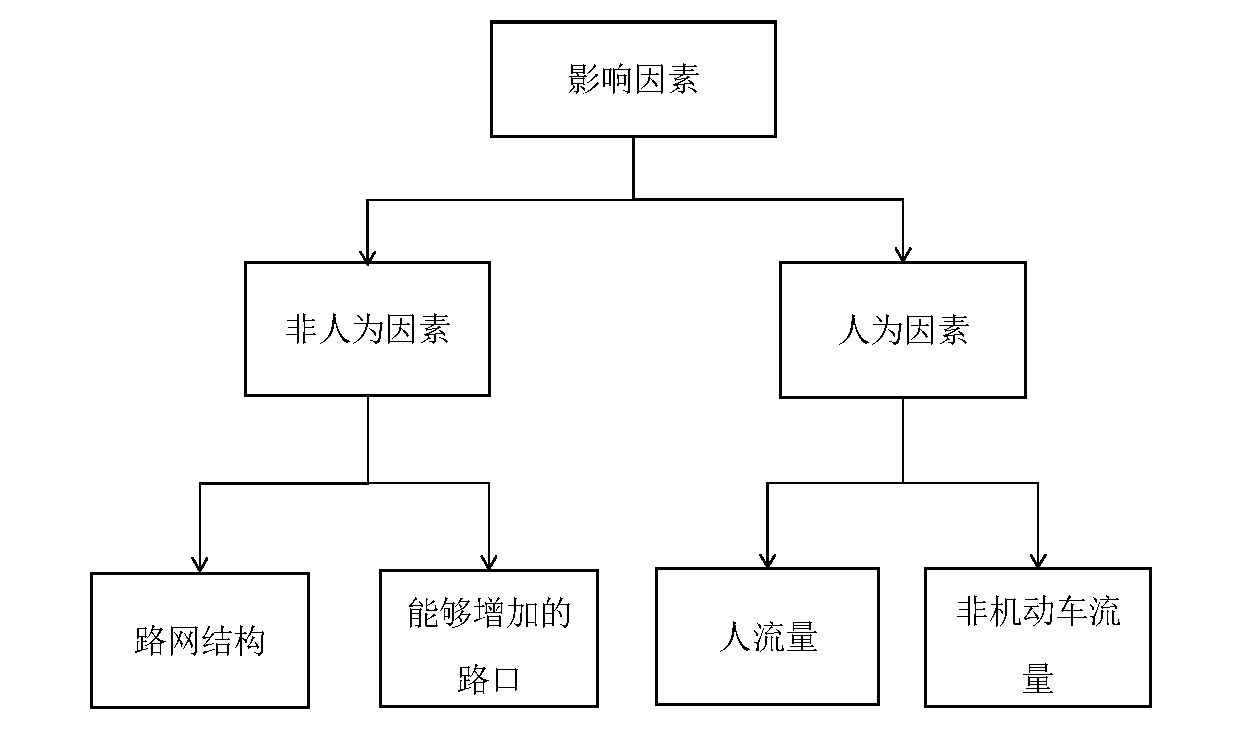
\includegraphics[width=0.7\textwidth]{pic/judge_result.pdf}
				\caption{影响因素的分层次结构}
				\label{fig:layer_struct}
			\end{figure}
			设影响因素的主因素集$ U=\{u_1,u_2,u_3\} $,评判等级集$ V=\{v_1,v_2,v_3\} $。
			其中$ U $中$ u_1 $代表路网结构改变对周边道路的影响,$ u_2 $代表人流量与非机动车流量对周边道路的影响,$ u_3 $代表可能增加的路口对周边道路造成的影响;$ V $中$ v_1 $代表开放小区对周边道路交通有积极影响,$ v_2 $代表开放小区对周边道路交通的改善效果一般,$ v_3 $代表开放小区对周边道路交通有不利影响。
			对U中每一个因素根据评判等级指标进行模糊评判,得到评判矩阵为:
			$$
				R=\left[
				\begin{array}{cccc}
					r_{11} & r_{12} & r_{13}\\
					r_{21} & r_{22} & r_{23}\\
					r_{31} & r_{32} & r_{33}
				\end{array}
				\right]
			$$
			其中$ r_{ij} $表示$ u_i $关于$ v_j $的隶属程度,则$ (U,V,R) $构成一个模糊评价模型,利用层次分析的方法确定各项因素的权重,比较影响因素集U中的元素,得到比较矩阵为:
			$$
				C=\left[
				\begin{array}{cccc}
					1 & 5 & 3\\
					1/5 & 1 & 1/2\\
					1/3 & 2 & 1
				\end{array}
				\right]
			$$
			得到C的特征向量$ D=[-0.9281,-0.1747,-0.3288] $,标准化之后为$ D=[0.6483 0.1220,0.2297]^Z $
			则评价模型中的权重因素记为$ A=D $,满足$ \sum_{i=1}^{3}a_i=1 $,
			合成得:
			\begin{equation}
				\overline{B}=A \cdot R=(\overline{b_1},\overline{b_2},\overline{b_3}) 
				\label{eq:judge_result}
			\end{equation}
			\ref{eq:judge_result}即是开放小区对周边交通影响的评价结果,其中$\overline{b_1},\overline{b_2},\overline{b_3}$分
			别代表主要因素对于评判等级的隶属度,归一化后我们还可以得到开放小区对周边的影响趋向某一个等级的程度即$ B=(b_1,b_2,b_3) $。

	\subsection{问题二}
		车辆通行时受到多方面因素的影响,我们通过建立模型得出车辆从起点到终点所用的时间,以此来分析开放小区对周边交通的影响。其中所用时间可以分为行驶在路上花费的行程时间,与因为其他因素造成的延误时间,所以车辆经过一段路程的总时间可以由\eqref{eq:time_total}表示,其中$ t_d $为延误时间,$t(q)$为路阻函数。
		\begin{equation}
			T = t_d + t(q)
			\label{eq:time_total}
		\end{equation}
		\subsubsection{延误时间}
			延误时间\upcite{任福田2003交通工程学}是指,道路上通行所需时间除行走时间外,也受市政道路交通信号灯的影响,如\eqref{eq:delay_func}所示。
			\begin{equation}
				t_d=\frac{0.5T(1-\frac{t_g}{T})}{1-[min(1,v/c)\cdot{\frac{t_g}{T}}]}
				\label{eq:delay_func}
			\end{equation}
			其中$ T $表示信号灯周期长度,$ t_g $代表绿灯时间,$ v,c $代表最大交通量与基本交通量。
			
		\subsubsection{行程时间}
			车辆行驶的行程时间主要受到道路阻抗的影响道路阻抗是表达车辆在运行过程中受到的阻碍程度的高低的量值,是城市交通网络研究中的重要参量,它直接影响交通流的路径选择和流量分配。
			
			美国联邦公路局路阻函数(即BPR函数)如\eqref{eq:bpr_plain}所示。
			\begin{equation}
				t(q)=t_0(1+\alpha(q/c)^\beta)
				\label{eq:bpr_plain}
			\end{equation}
			其中$ t(q) $表示流量为q时该路段的行程时间,$ t_0 $为该路段的自由流行程时间,$ c $为该路段上的实际通行能力,$ \alpha,\beta $为回归系数,一般取$ \alpha=0.15,\beta=4 $由于模型中的c并不具有固定的含义\upcite{郑远2007美国联邦公路局路阻函数探讨},我们采取修正过的BPR函数并对其改进
			,考虑到小区内道路上行人、自行车等非机动车较多的
			特点,增加行人对机动车的影响、自行车对机动车的影响。结合已有的研究成果\upcite{李向朋2014城市交通拥堵对策—封闭型小区交通开放研究},得到行人干扰修正系数如表\ref{tab:walker_noise}。
			
			非机动车对车辆的影响系数由\eqref{eq:bike}得到。
			\begin{table}[!htbp]
				\centering
				\caption{行人干扰的修正系数}
				\label{tab:walker_noise}
				\begin{tabular}{c|cccccc}
					\hline 
					干扰程度 & 很严重 & 严重 & 较严重 & 无 & 很小 & 一般 \\ 
					\hline 
					$\eta$ & 0.5 & 0.6 & 0.7 & 1.0 & 0.9 & 0.8 \\ 
					\hline 
				\end{tabular}
			\end{table}
			\begin{equation}
				\eta_b = 0.8-\frac{(q_b/Q_b+0.5-W_2)}{W_1}
				\label{eq:bike}
			\end{equation}
			其中$ \eta_b $非机动车干扰系数,$ q_b $非机动车流量,$ Q_b $非机动车道通行能力$ W_1,W_2 $
			非机动车道宽度与机动车道宽度。
			
			综上所述,得到改进BPR路阻函数如\eqref{eq:bpr_imporve}。
			\begin{equation}
				t(q)=\left\lbrace
				\begin{array}{lr}
					t_0(1+\alpha(\frac{qv}{c\eta\eta_b})^\beta) & 0\leq\eta_b\leq1\\
					t_0(1+\alpha(\frac{\eta_bqv}{c\eta})^\beta) & 1\leq\eta_b
				\end{array}	
				\right.
				\label{eq:bpr_imporve}
			\end{equation}			
			则\eqref{eq:time_total}可以表示为\eqref{eq:time_final}所示形式。
			\begin{equation}
				T=\left\lbrace
				\begin{array}{lr}
					t_0(1+\alpha(\frac{qv}{c\eta\eta_b})^\beta)+\frac{0.5T(1-\frac{t_g}{T})}{1-[min(1,v/c)\cdot{\frac{t_g}{T}}]} & 0\leq\eta_b\leq1\\
					t_0(1+\alpha(\frac{\eta_bqv}{c\eta})^\beta)+\frac{0.5T(1-\frac{t_g}{T})}{1-[min(1,v/c)\cdot{\frac{t_g}{T}}]} & 1\leq\eta_b
				\end{array}	
				\right.
				\label{eq:time_final}
			\end{equation}
		\subsubsection{动态交通分配理论}
			交通分配是指根据现有道路网络,按照一定规则将进入交通网络的流量合理地分配道网路中的各个道路上,并由此得到网络中各个路段的数据。交通流量是随时间变化的,这要求对于交通流的分配也应该具有动态性\cite{陆化普1996动态交通分配理论的回顾与展望},
			
			
		\subsubsection{Braess悖论}
			数学家Dietrich Braess在1968年首次提出了Braess悖论\upcite{Braess1968Ü}。
			考虑拓扑结构如图\ref{fig:braess}的交通网,假设交通网中的流量为4000,起点为A,终点为D
			通过$ A \rightarrow B $与$ C \rightarrow D $的时间均为车流量除以100,通
			过$ B \rightarrow D $与$ A \rightarrow C $的时间为固定的45分钟。
			\begin{figure}[!htbp]
				\centering
				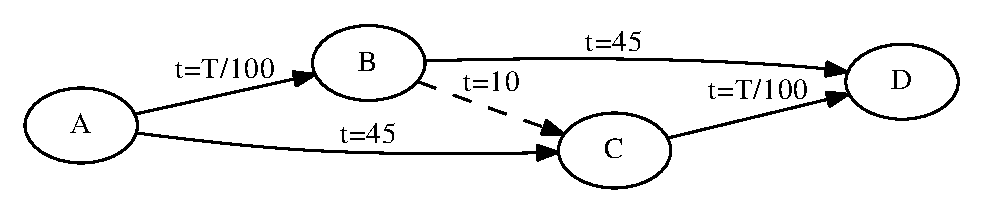
\includegraphics[width=0.5\textwidth]{pic/braess.eps}
				\caption{Braess悖论的具体情况}
				\label{fig:braess}
			\end{figure}
			在路径$ B \rightarrow C $没有开通时,从$ A \rightarrow D $的通过时间分别为$ \frac{A}{100}+45 $与$ \frac{B}
			{100} + 45 $,达到均衡之后有$ A=B=2000 $这样每条路通过的时间都是$ \frac{2000}{100}
			+45=65 $分钟。
			
			现在考虑$ B \rightarrow C $开通之后,其通过时间非常短,在这种情况下,所有司机都会选择$ A \rightarrow B \rightarrow C \rightarrow D $这条路线,因为即使所有车辆全部通过$ A \rightarrow B $所用时间也不超过40分钟,这样所有通过这条路径的时间为$ \frac{4000}{100}\times 2+10=90$分钟,Braess悖论便是指这种情况。
			\subsubsection{基于Braess的评价系统}
			小区开放相当与在原有的交通网络中再次加入新的网路,其中必然会有某些情况导致Braess悖论的发生,而出现这种情时况不宜开放小区。
			
			查阅论文可知Pas和Principcipio在其论文中指出了Braess悖论不发生的两种情况\upcite{pas1997braess},一种时交通量低时,如\ref{eq:Q_low},另一种时交通量高时\ref{eq:Q_high},当交通量符合上述两种情况时,不发生Braess现象,如\ref{eq:Q_mid}所示。
			\begin{equation}
			Q>\frac{2(\alpha_n-\alpha_x)}{3\beta_n+\beta_x}
				\label{eq:Q_low}
			\end{equation}
			\begin{equation}
				Q<\frac{2(\alpha_n-\alpha_x)}{\beta_n-\beta_x}
				\label{eq:Q_high}
			\end{equation}
			\begin{equation}
			\frac{2(\alpha_n-\alpha_x)}{3\beta_n+\beta_x}<Q<\frac{2(\alpha_n-\alpha_x)}{\beta_n-\beta_x}
			\label{eq:Q_mid}
			\end{equation}
			其中$ Q $为交通需求,		
	\subsection{问题二}
		综合问题一的评价模型建立元胞自动机模型
		\begin{equation}
			A=(L,d,S,N,f)
		\end{equation}
		其中A代表自动机模型,其中L为元胞空间;d为元胞空间的维数;S为状态集合;N为某个邻域内所有元胞的集合;f为局部映射或局部规则。
		根据问题一中的模型,建立一个二维元胞自动机模型,每个每个元胞具有几个固定的生成地点,在
		$ L $中有确定的目的地。
  \newpage
  \bibliography{mybib}
  \bibliographystyle{gbt7714}

\end{document}